\documentclass[10pt,a4paper,oneside]{article}
\usepackage{cmap}
\usepackage[T2A]{fontenc}
\usepackage{float}
\usepackage{listings}
\usepackage{csquotes}
\usepackage[utf8]{inputenc}
\usepackage{amsmath}
\usepackage{amsfonts}
\usepackage{amssymb}
\usepackage[english, russian]{babel}%Подключаем русский язык.
\usepackage{graphicx}
\usepackage{geometry} % Меняем поля страницы.
\geometry{left=3cm} %Левое поле.
\geometry{right=2cm} %Правое поле.
\geometry{top=3cm} %Верхнее поле.
\geometry{bottom=2cm} %Нижнее поле.


%Начало документа
\begin{document}

%Создаём титульник.
\begin{titlepage}
\newpage
	%Название ВУЗа и институт.
	\begin{center}
		\Large Санкт-Петербургский Государственный Политехнический Университет\\
		Институт Компьютерных Наук и Технологий\\
	\end{center}
	%Кафедра.
	\begin{center}
		\large\textbf {Высшая школа интеллектуальных систем и суперкомпьютерных технологий}
	\end{center}
	
	%Пропуск места. 
	\vspace{5em}
	%!!!!!!!!!!!!!!!!!!!!!!!!!!!!!!!!!Название работы.
	\begin{center}
		\large{Отчёт по лабораторной работе №5 \\ на тему \\
		\textbf{Автокорреляция} }
	\end{center}
	
	%Делаем пропуск и пишем студента и преподавателя.
	\vspace{25em}
	\begin{flushright}
		\textbf{Работу выполнил\\}Студент группы 3530901/80203 \\ Тарасенко Н.С.\\
		\textbf{Преподаватель\\}Богач Н.В. 
	\end{flushright}
	
	\vspace{\fill}%В самом низу
	\begin{center}
	Санкт-Петербург, 2021 год	
	\end{center}
\end{titlepage} %Закончили титульный лист.

\section{Настройка проекта}
Перед тем как выполнять задания необходимо настроить проект и сделать все необходимые импорты:

\begin{figure}[H]
        \centering
        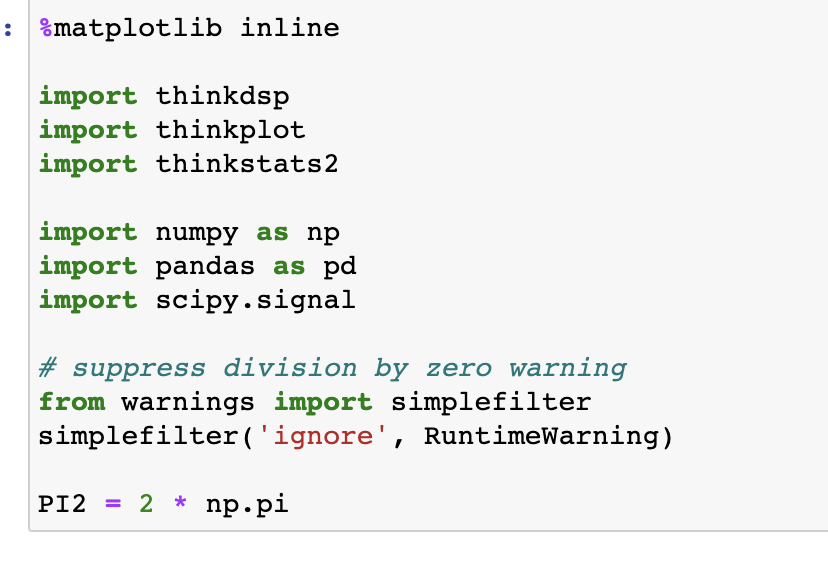
\includegraphics[width=0.75\textwidth]{0.png}
        \caption{2}
        \label{fig:first}
\end{figure}

\section{Упражнение номер №1}

Необходимо оценить высоты тона вокального чирпа для нескольких времен начала сегмента.

Возьмем методы из chap05.ipynb

\begin{figure}[H]
        \centering
        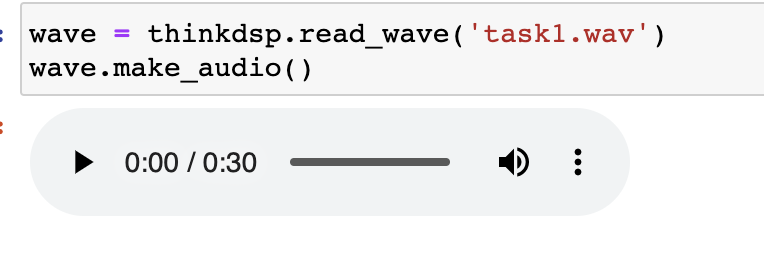
\includegraphics[width=0.75\textwidth]{1.png}
        \caption{2}
        \label{fig:first}
\end{figure}

Возьмем звук из репозитория и выделим из него короткий сегмент. Применим для этого сегмента функцию автокорреляции, чтобы оценить высоту тона: 

\begin{figure}[H]
        \centering
        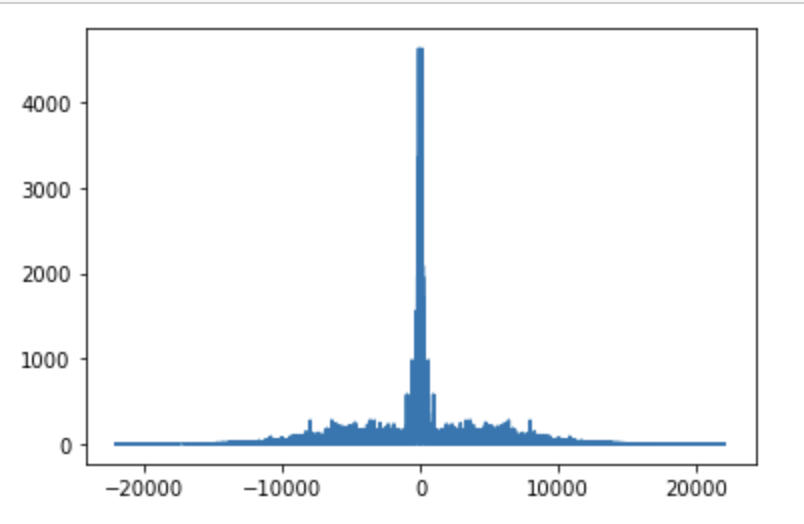
\includegraphics[width=0.75\textwidth]{2.png}
        \caption{2}
        \label{fig:first}
\end{figure}

Пик ∈ [100;150]. Используем argmax, чтобы уточнить значение для этого пика

\begin{figure}[H]
        \centering
        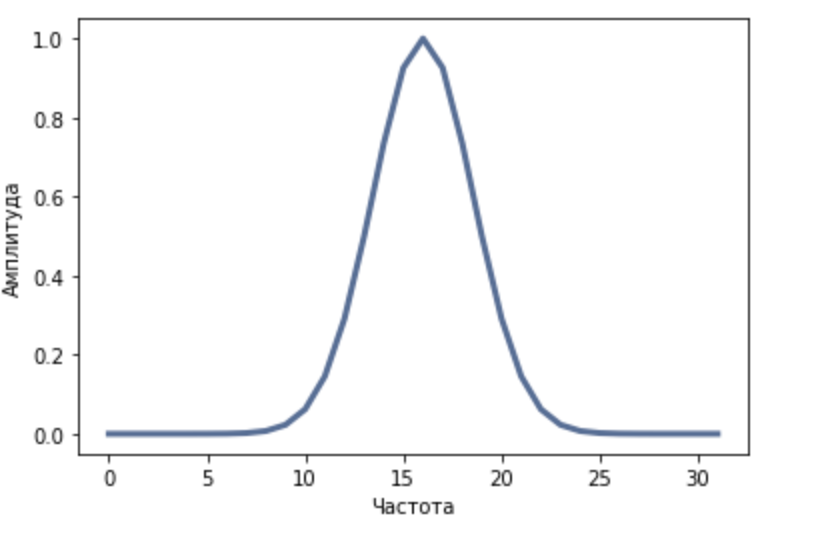
\includegraphics[width=0.75\textwidth]{3.png}
        \caption{2}
        \label{fig:first}
\end{figure}
Вычислим частоту для этого значения: 

\begin{figure}[H]
        \centering
        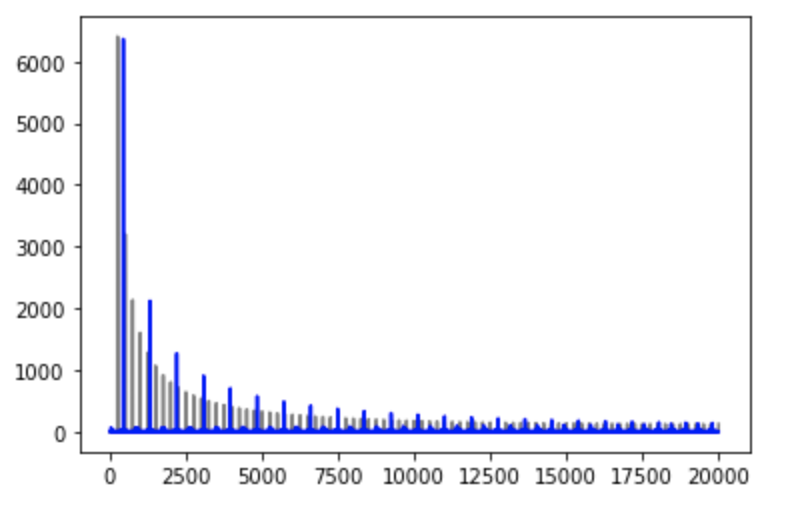
\includegraphics[width=0.75\textwidth]{4.png}
        \caption{2}
        \label{fig:first}
\end{figure}

Возьмем другой сегмент и проделаем те же манипуляции: 

\begin{figure}[H]
        \centering
        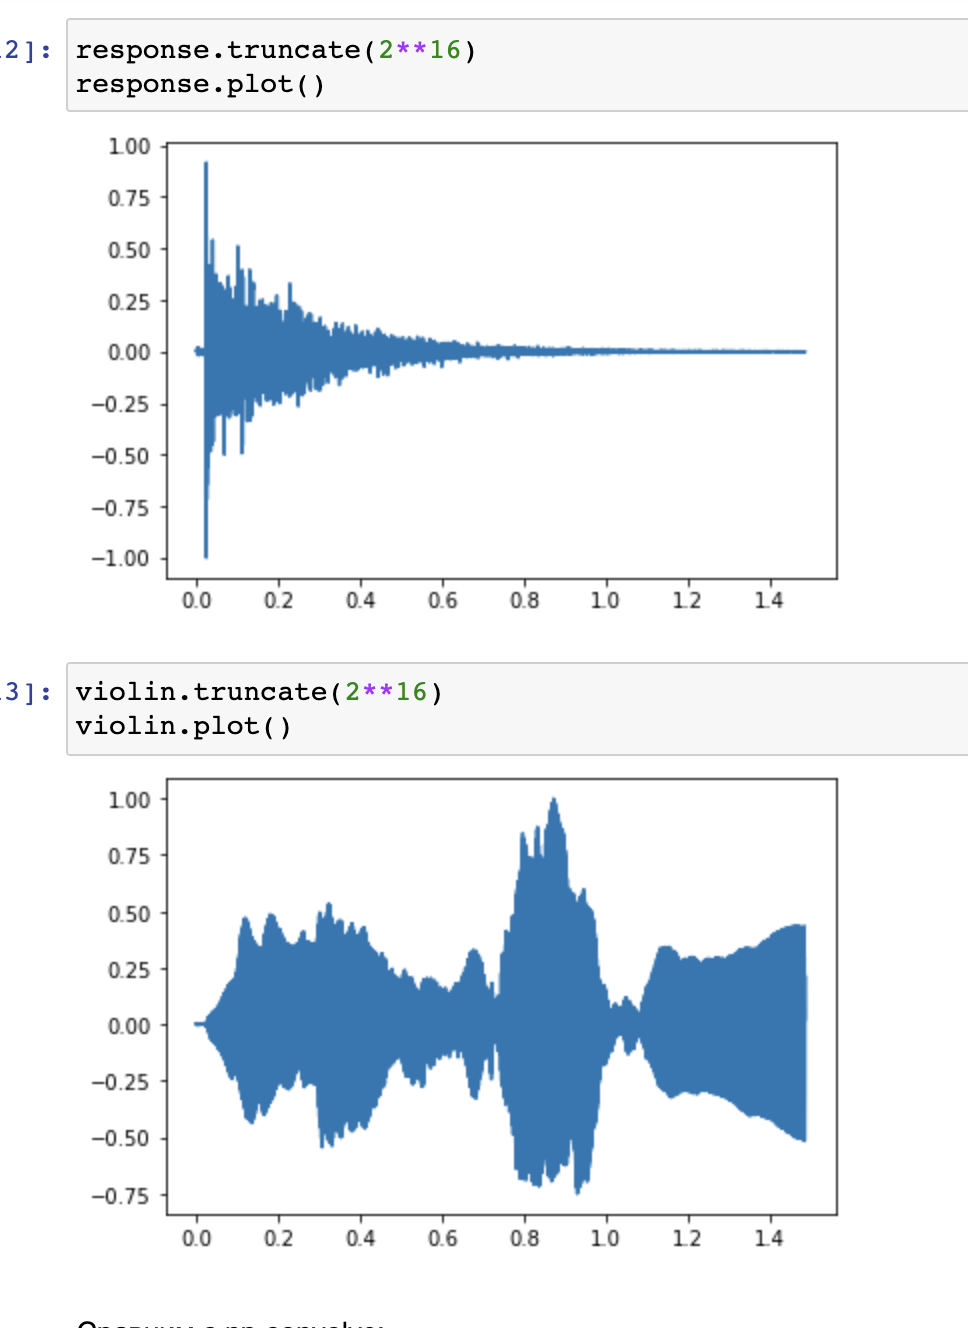
\includegraphics[width=0.75\textwidth]{5.png}
        \caption{2}
        \label{fig:first}
\end{figure}

Пик ∈ [100;150]. Используем argmax, чтобы уточнить значение для этого пика

\begin{figure}[H]
        \centering
        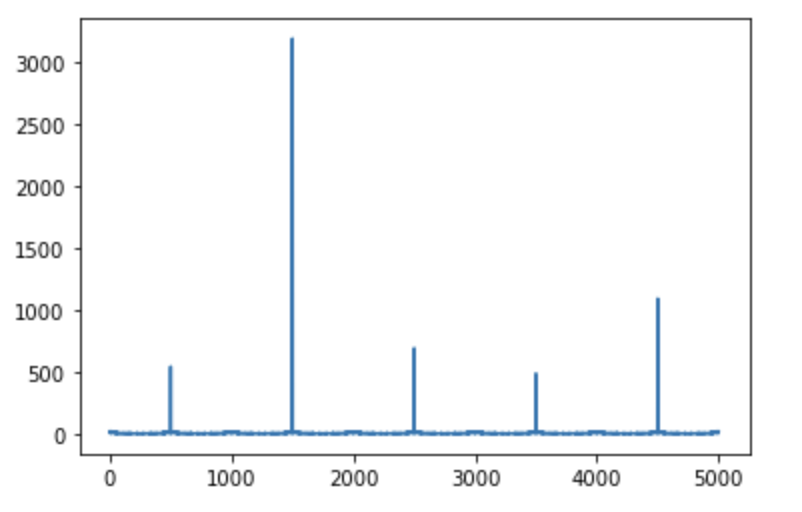
\includegraphics[width=0.75\textwidth]{6.png}
        \caption{2}
        \label{fig:first}
\end{figure}

Вычислим частоту для этого значения: 

\begin{figure}[H]
        \centering
        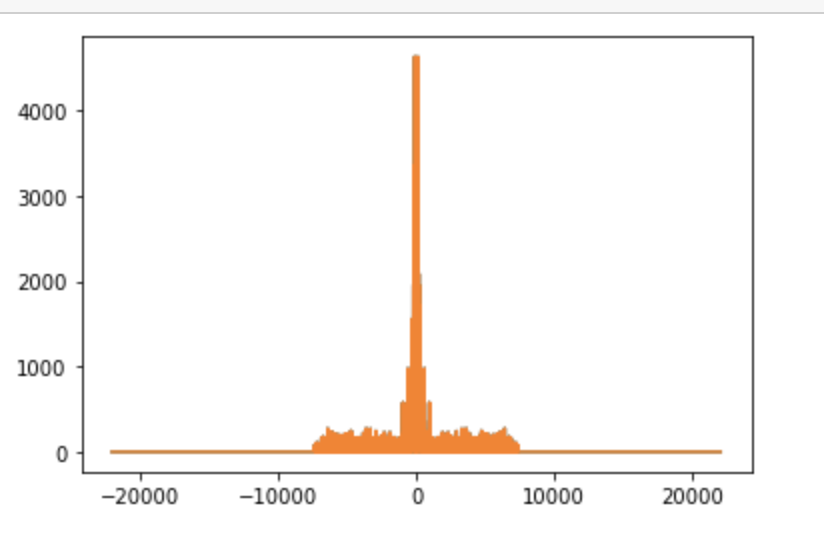
\includegraphics[width=0.75\textwidth]{7.png}
        \caption{2}
        \label{fig:first}
\end{figure}

Делаем вывод, что частота обратно пропорциональна времени начала сегмента

\section{Упражнение номер №2}

Инкапуслировать код в функцию из преложенного кода, назвав ее estimate_fundamental. Использовать жту функцию для отслеживания высоты тона записанного звука. Проверить насколько она хорошо работает, накладывая оценки высоты тона на спектрограмму записи.

Возьмем тот же звук что и в упражении 1. Распечатаем спектрограмму: 

\begin{figure}[H]
        \centering
        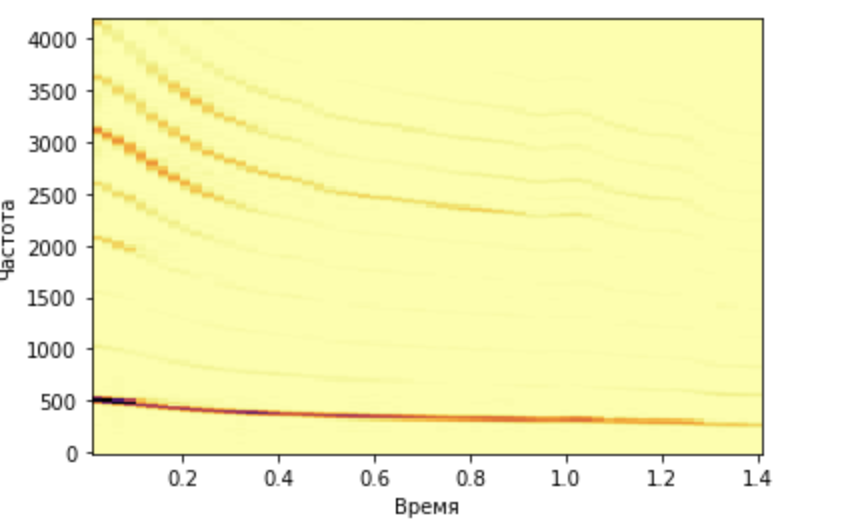
\includegraphics[width=0.75\textwidth]{8.png}
        \caption{2}
        \label{fig:first}
\end{figure}

Упростим задачу, указав диапазон Lag для поиска, так как найти самый первый высокий пик достаточно сложно.

Реализуем функцию: 

\begin{figure}[H]
        \centering
        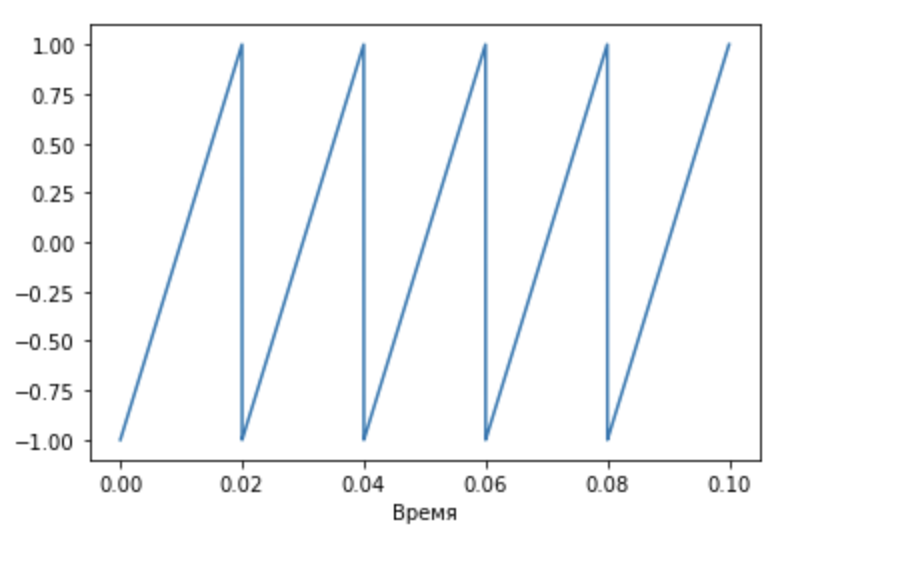
\includegraphics[width=0.75\textwidth]{9.png}
        \caption{2}
        \label{fig:first}
\end{figure}

Рассмотрим пример использования данной функции: 

\begin{figure}[H]
        \centering
        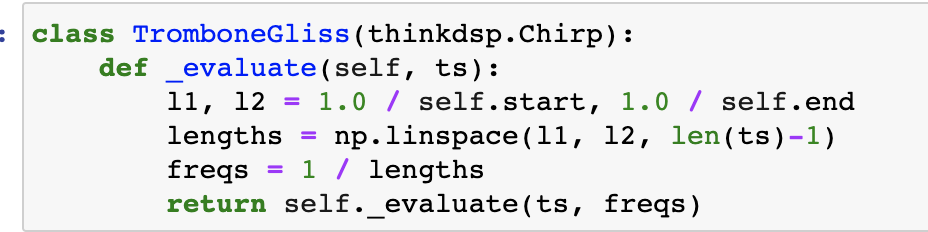
\includegraphics[width=0.75\textwidth]{10.png}
        \caption{2}
        \label{fig:first}
\end{figure}

Используем функцию для отслеживания высоты звука по сэмплу. Ts - это средние точки каждого сегмента.

\begin{figure}[H]
        \centering
        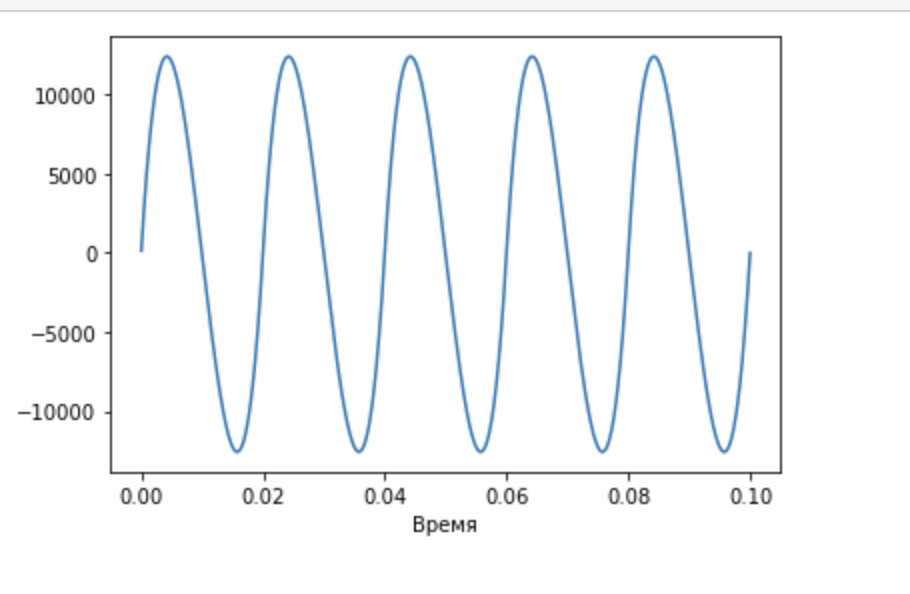
\includegraphics[width=0.75\textwidth]{11.png}
        \caption{2}
        \label{fig:first}
\end{figure}

Вот кривая для отслеживания высоты тона, наложенная на спектрограмму:

\begin{figure}[H]
        \centering
        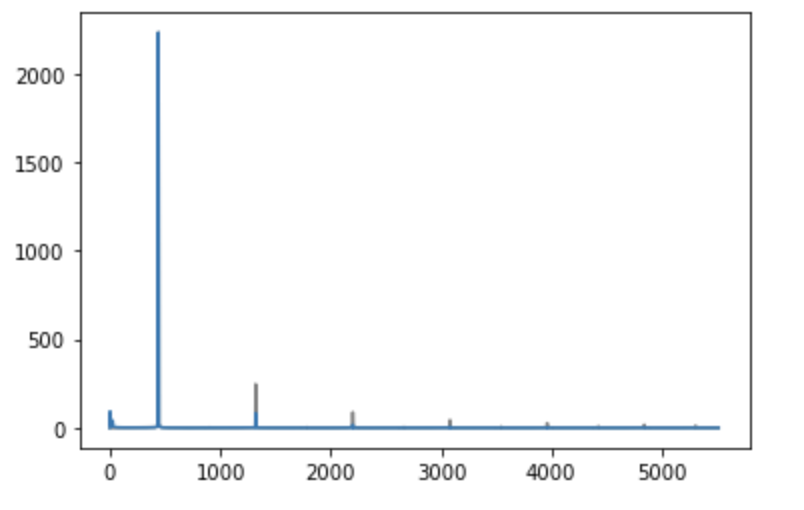
\includegraphics[width=0.75\textwidth]{12.png}
        \caption{2}
        \label{fig:first}
\end{figure}

\section{Упражнение номер №3}

Вычилсить автокорреляцию цен в платежной системе биткоина. 

Возьмем те же данные, что и в прошлой главе: 

\begin{figure}[H]
        \centering
        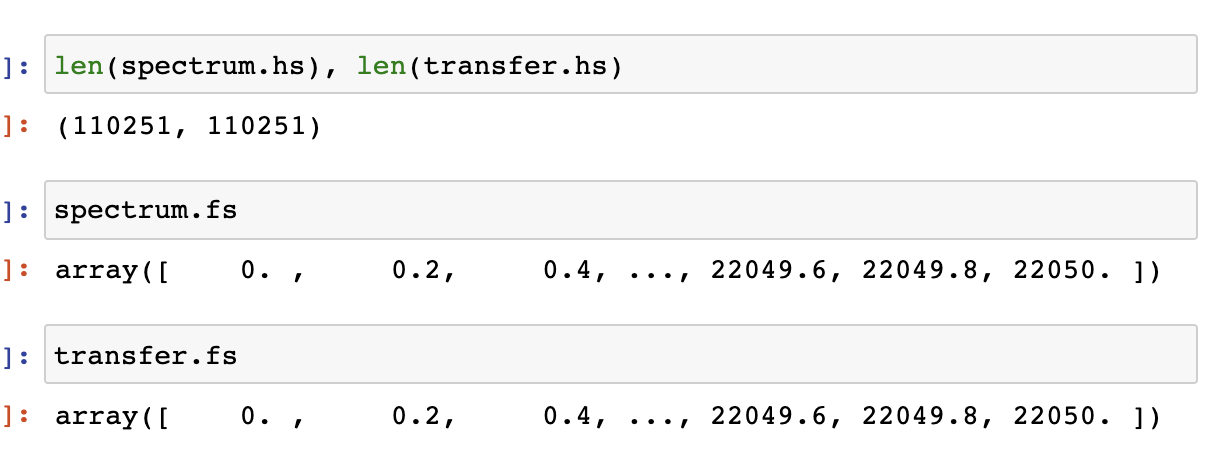
\includegraphics[width=0.75\textwidth]{13.png}
        \caption{2}
        \label{fig:first}
\end{figure}

Построим волну: 

\begin{figure}[H]
        \centering
        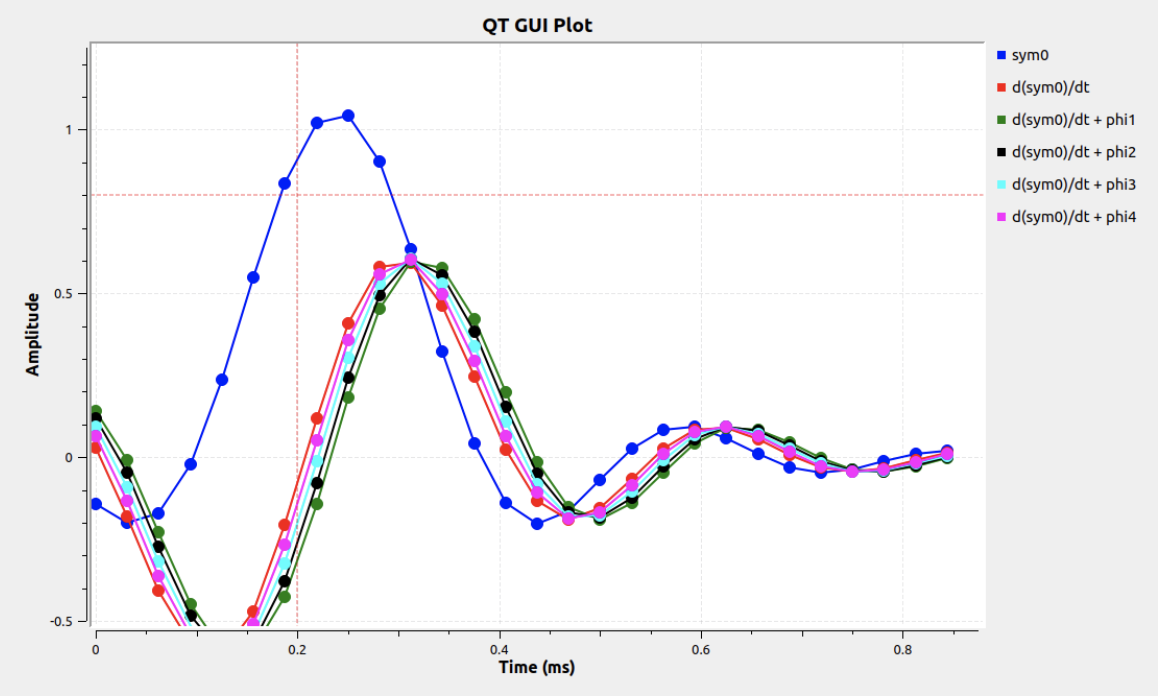
\includegraphics[width=0.75\textwidth]{14.png}
        \caption{2}
        \label{fig:first}
\end{figure}

Применим функцию автокорреляции: 

\begin{figure}[H]
        \centering
        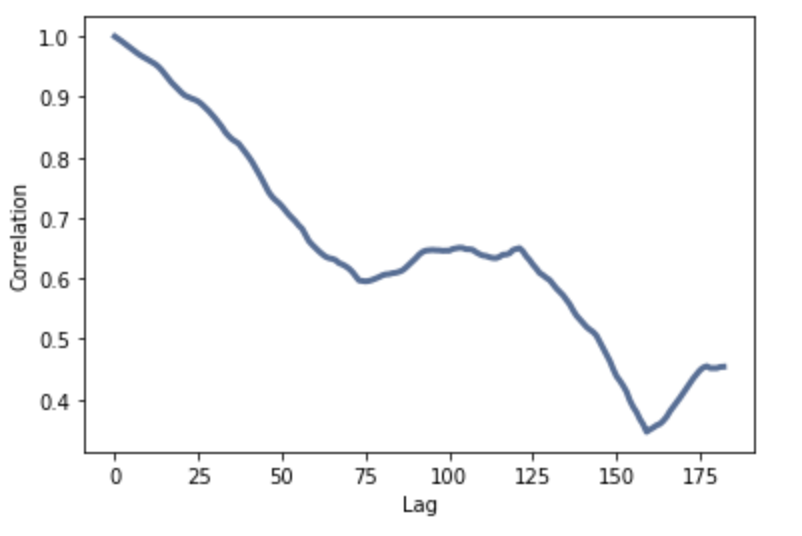
\includegraphics[width=0.75\textwidth]{15.png}
        \caption{2}
        \label{fig:first}
\end{figure}

Функция медленно снижается по мере увеличения задержки, что указывает на какой-то розовый шум.

Мы можем сравнить autocorr с np.correlate, в котором используется определение корреляции, используемое при обработке сигналов. Он не устраняет предвзятость, нормализует и не стандартизирует волну.

\begin{figure}[H]
        \centering
        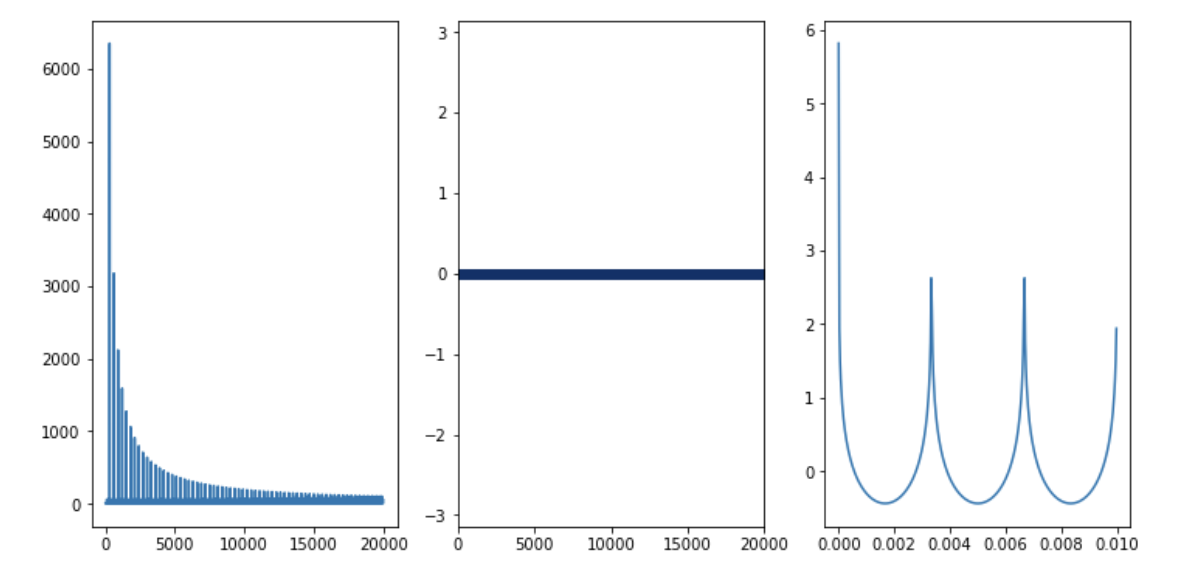
\includegraphics[width=0.75\textwidth]{16.png}
        \caption{2}
        \label{fig:first}
\end{figure}

Вторая половина результата соответствует положительным Lags:

\begin{figure}[H]
        \centering
        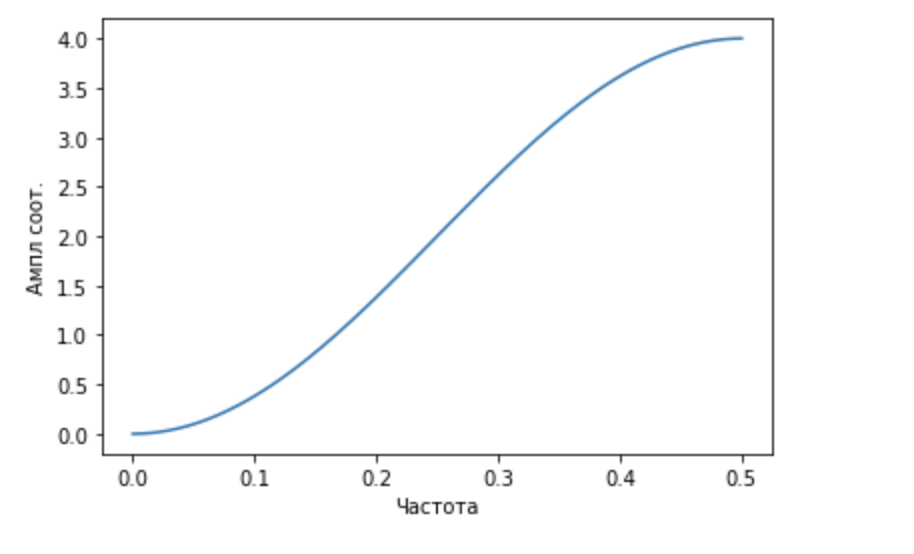
\includegraphics[width=0.75\textwidth]{17.png}
        \caption{2}
        \label{fig:first}
\end{figure}

Нормализуем результаты постфактум, разделив их по длине:

\begin{figure}[H]
        \centering
        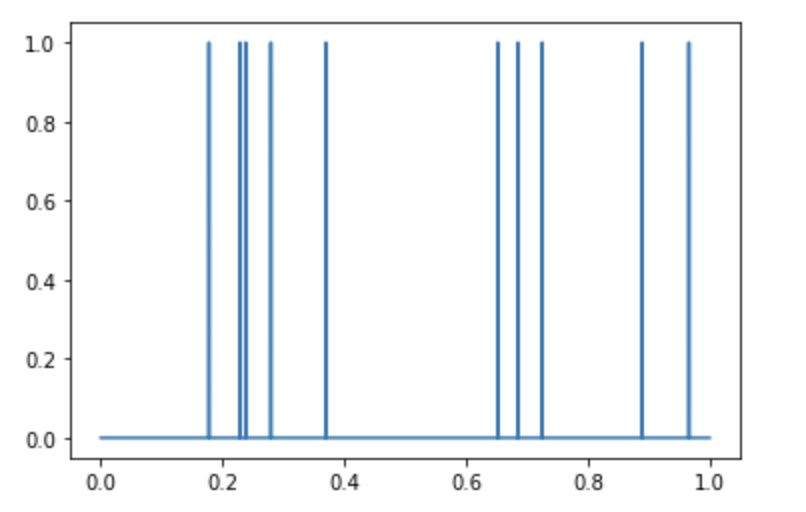
\includegraphics[width=0.75\textwidth]{18.png}
        \caption{2}
        \label{fig:first}
\end{figure}

Наложим и сравним полученные результаты: 

\begin{figure}[H]
        \centering
        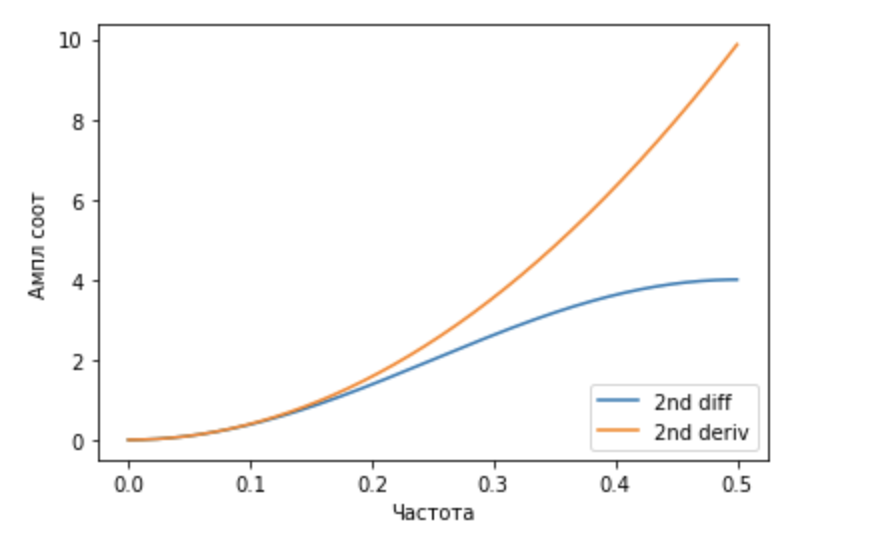
\includegraphics[width=0.75\textwidth]{19.png}
        \caption{2}
        \label{fig:first}
\end{figure}

Даже после стандартизации результаты выглядят существенно иначе.

Для этого набора данных, вероятно, более подходящим является статистическое определение ACF.

\section{Упражнение номер №4}

Изучить предложенный файл saxophone.ipynb

Сделаем необходимые импорты: 

\begin{figure}[H]
        \centering
        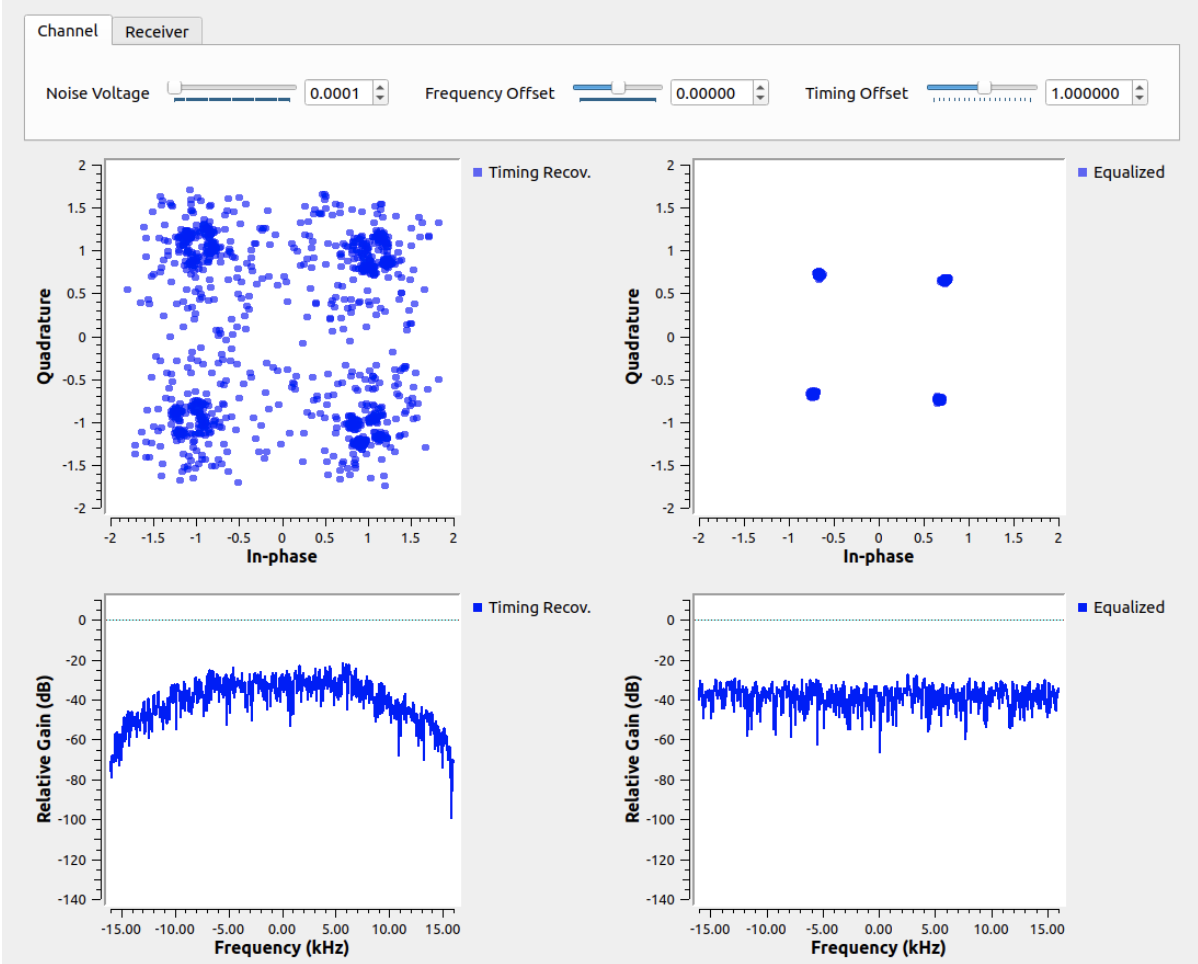
\includegraphics[width=0.75\textwidth]{20.png}
        \caption{2}
        \label{fig:first}
\end{figure}

Возьмем звук, предложенный учебником и выведем спектрограмму: 

\begin{figure}[H]
        \centering
        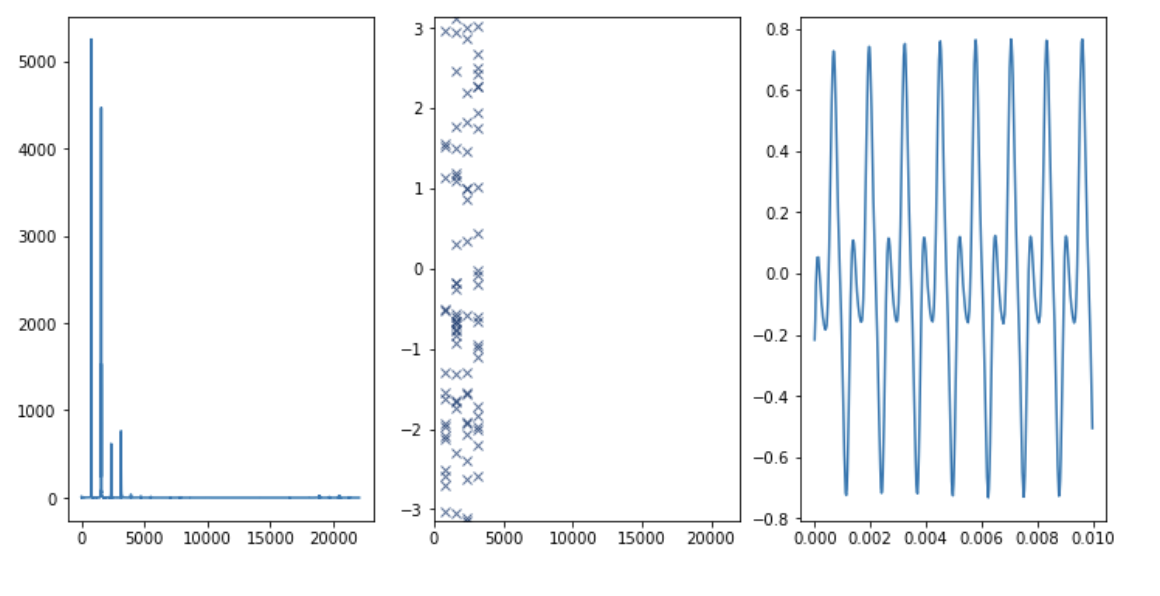
\includegraphics[width=0.75\textwidth]{21.png}
        \caption{2}
        \label{fig:first}
\end{figure}

Спектрограмма показывает гармоническую структуру во времени.

Выберем сегмент, чтобы лучше увидеть гармоники и выведем его спектр:

\begin{figure}[H]
        \centering
        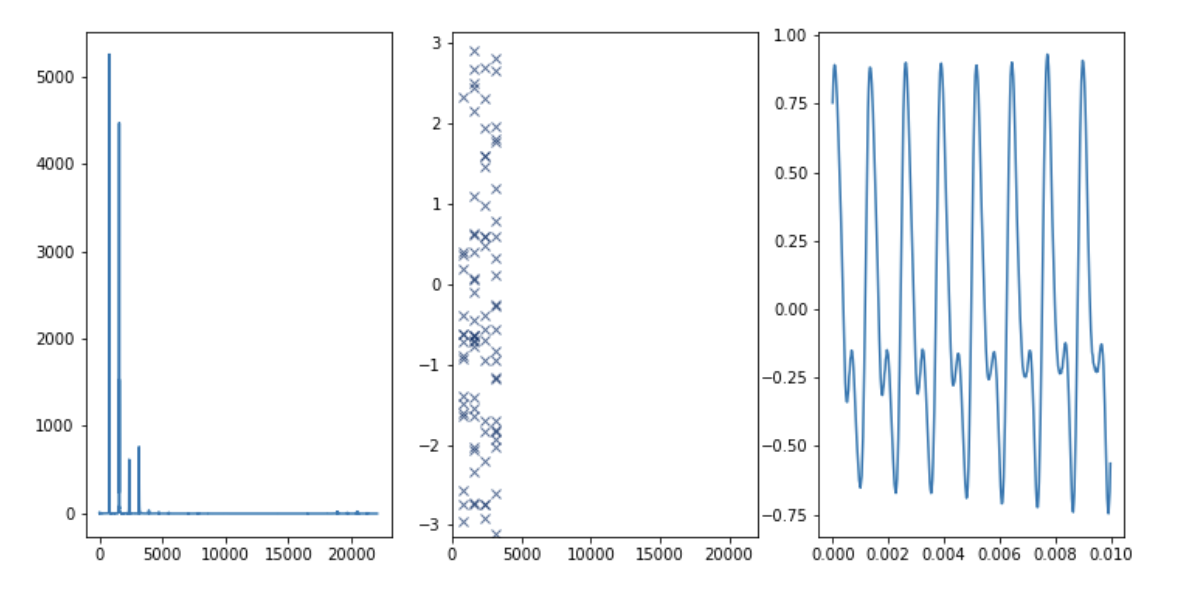
\includegraphics[width=0.75\textwidth]{22.png}
        \caption{2}
        \label{fig:first}
\end{figure}

Пики в спектре находятся на частотах 1392, 928 и 464 Гц.

\begin{figure}[H]
        \centering
        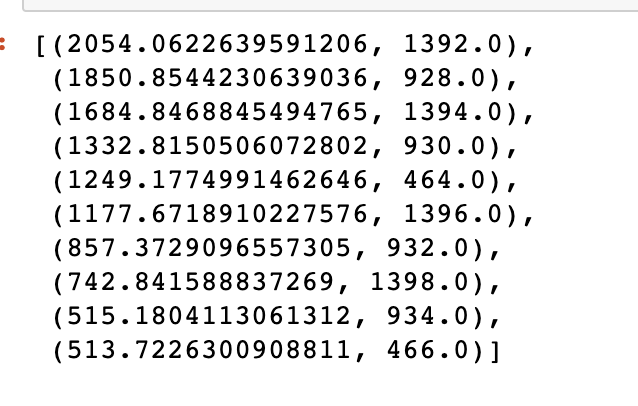
\includegraphics[width=0.75\textwidth]{23.png}
        \caption{2}
        \label{fig:first}
\end{figure}

Высота, которую мы воспринимаем, является основной, 464 Гц, хотя это не доминирующая частота.

Для сравнения, вот треугольная волна на частоте 464 Гц.

\begin{figure}[H]
        \centering
        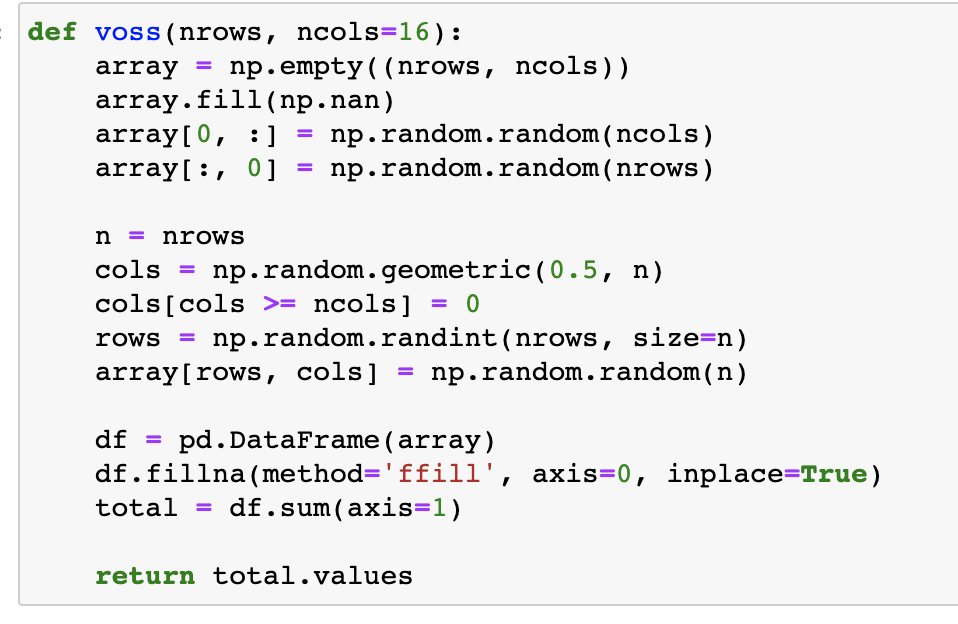
\includegraphics[width=0.75\textwidth]{24.png}
        \caption{2}
        \label{fig:first}
\end{figure}

У них одинаковая воспринимаемая высота звука.

Чтобы понять, почему мы воспринимаем основную частоту, даже если она не является доминирующей, полезно взглянуть на функцию автокорреляции (ACF).

Следующая функция вычисляет ACF, выбирает вторую половину (которая соответствует положительным задержкам) и нормализует результаты:

\begin{figure}[H]
        \centering
        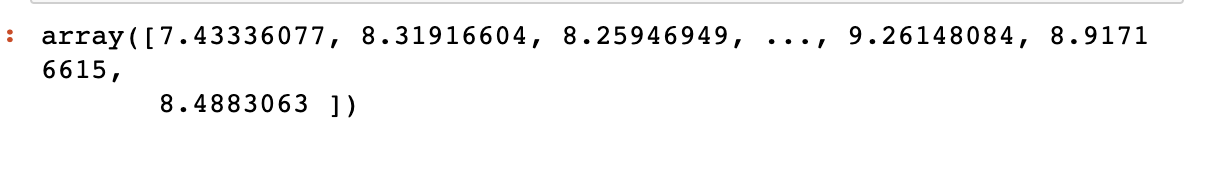
\includegraphics[width=0.75\textwidth]{25.png}
        \caption{2}
        \label{fig:first}
\end{figure}

Первый главный пик находится рядом с лагом 100.

Следующая функция находит самую высокую корреляцию в заданном диапазоне задержек и возвращает соответствующую частоту.

\begin{figure}[H]
        \centering
        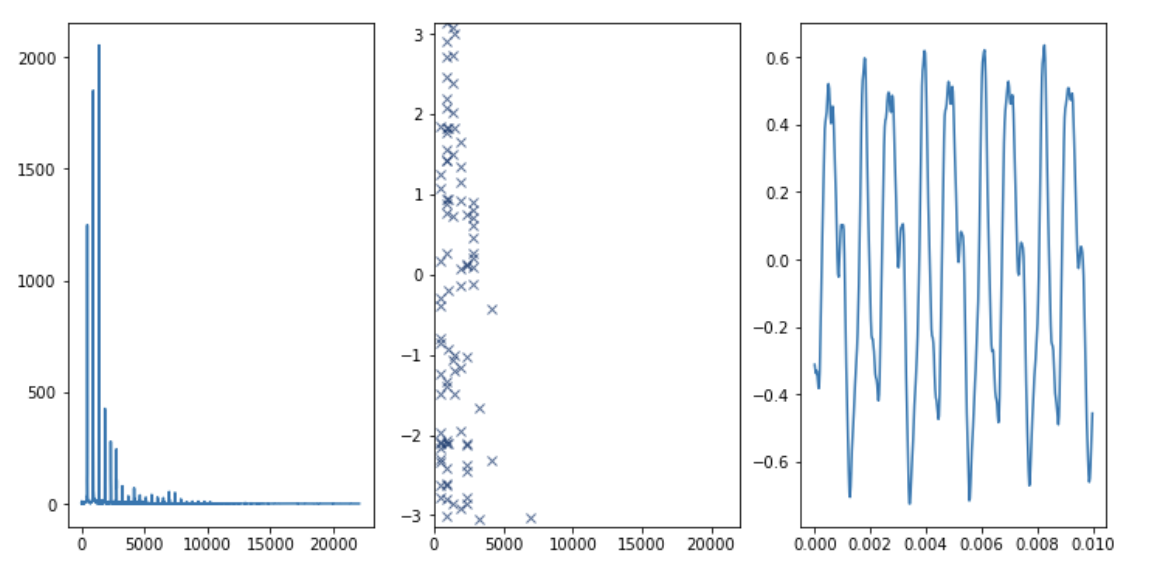
\includegraphics[width=0.75\textwidth]{26.png}
        \caption{2}
        \label{fig:first}
\end{figure}

Наибольший пик приходится на lag 95, что соответствует частоте 464.21 Гц. По крайней мере, в этом примере высота звука, которую мы воспринимаем, соответствует наивысшему пику автокорреляционной функции (ACF), а не самому высокому компоненту спектра. Удивительно, но воспринимаемый шаг не меняется, если мы полностью удаляем фундаментальный. Вот как выглядит спектр, если мы используем фильтр высоких частот, чтобы убрать фундаментальный.

Выведем спектр: 

\begin{figure}[H]
        \centering
        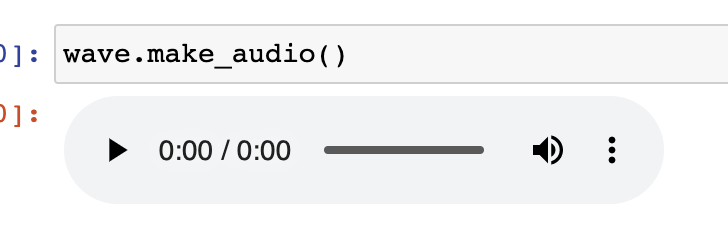
\includegraphics[width=0.75\textwidth]{27.png}
        \caption{2}
        \label{fig:first}
\end{figure}

Создадим звук. Воспринимаемая высота звука по-прежнему составляет 464 Гц, хотя на этой частоте нет мощности.

Чтобы понять, почему мы слышим частоту, которой нет в сигнале, полезно взглянуть на функцию автокорреляции (ACF).

\begin{figure}[H]
        \centering
        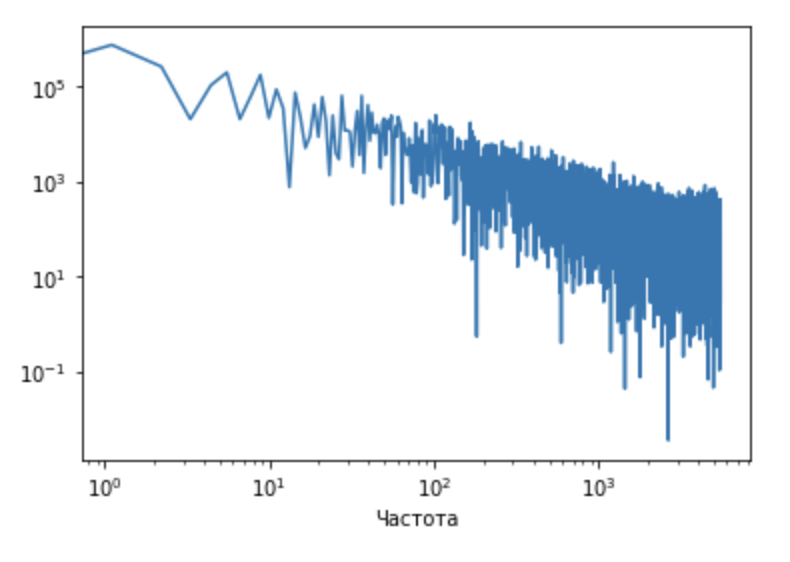
\includegraphics[width=0.75\textwidth]{28.png}
        \caption{2}
        \label{fig:first}
\end{figure}

Третий пик, соответствующий 464 Гц, по-прежнему самый высокий:

\begin{figure}[H]
        \centering
        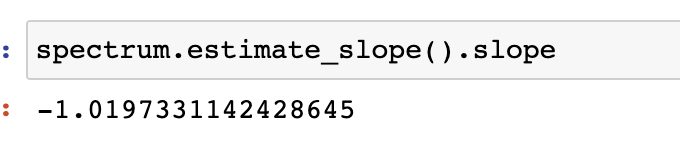
\includegraphics[width=0.75\textwidth]{29.png}
        \caption{2}
        \label{fig:first}
\end{figure}

Остальные пики не являются гармониками.

Наше ухо интерпретирует высокие гармоники как свидетельство того, что "правильный" фундаментал находится на частоте 464 Гц.

Если мы избавимся от высоких гармоник, эффект исчезнет. Рассмотрим спектр с удалёнными гармониками выше 1200 Гц.

\begin{figure}[H]
        \centering
        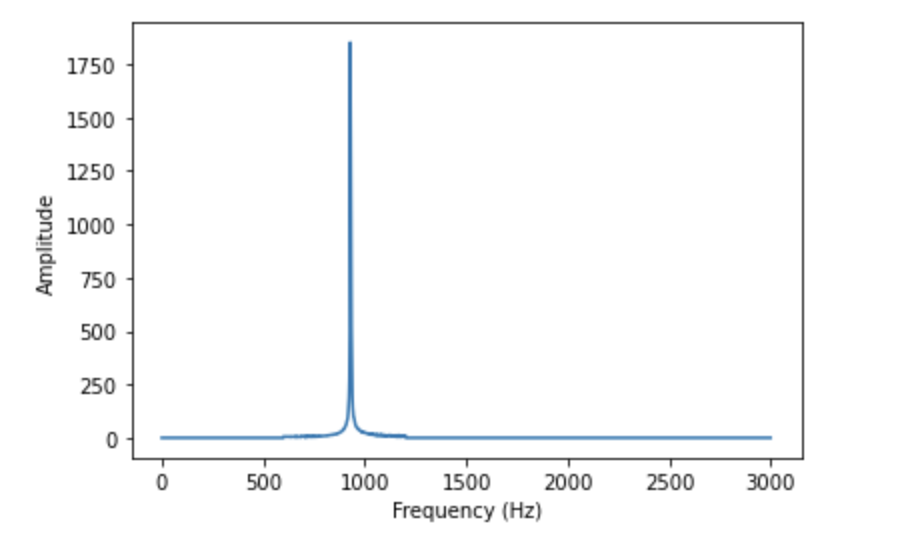
\includegraphics[width=0.75\textwidth]{30.png}
        \caption{2}
        \label{fig:first}
\end{figure}

Сейчас воспринимается частота примерно равная 930Гц. Создадим треугольный сигнал. И если мы посмотрим на функцию автокорреляции, мы найдем самый высокий пик при лаге = 47, что соответствует 938 Гц.

\begin{figure}[H]
        \centering
        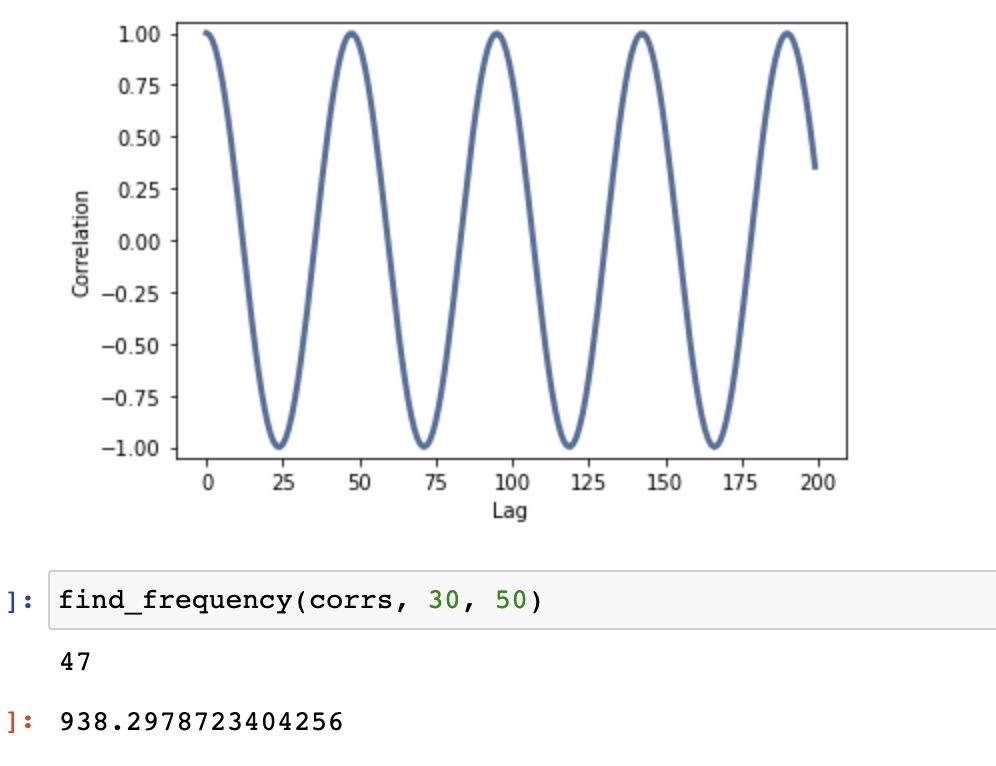
\includegraphics[width=0.75\textwidth]{31.png}
        \caption{2}
        \label{fig:first}
\end{figure}

\end{document}